% --- The evaluation landscape ---
\begin{frame}{Two Axes That Organise Almost Every Benchmark}
  \begin{itemize}\footnotesize\itemsep0.3em
    \item[\textcolor{red}{$\blacktriangleright$}] \textbf{Where do the questions come from?} A \textbf{static} dataset frozen at release, or a \textbf{live} stream of fresh items that a model could not have seen.
    \item[\textcolor{red}{$\blacktriangleright$}] \textbf{What decides whether the answer is good?} An objective \textbf{ground truth} (a key, a unit test, a compiler), or a \textbf{human preference} judgment (or a model standing in for one).
  \end{itemize}
  \vspace{0.2em}
  {\centering
  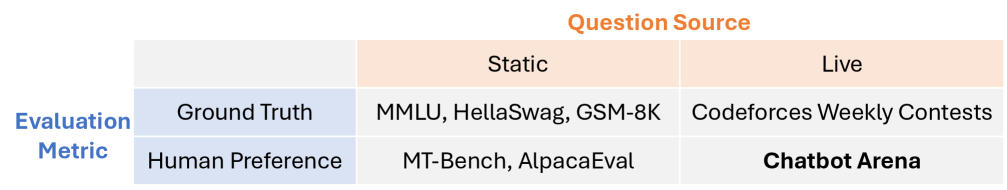
\includegraphics[width=0.9\textwidth,height=0.4\textheight,keepaspectratio]{images/llm-evaluation/arena_fig1_benchmark_taxonomy.png}\\[0.2em]
  {\scriptsize Chiang et al., ``Chatbot Arena: An Open Platform for Evaluating LLMs by Human Preference,'' \href{https://arxiv.org/abs/2403.04132v1}{arXiv:2403.04132v1}, Figure 1.}\par}
  \vspace{0.2em}
  \begin{itemize}\footnotesize
    \item[\textcolor{red}{$\blacktriangleright$}] The four quadrants have different failure modes. Static + ground truth is cheap and reproducible but \textbf{contaminable}; live + human preference resists contamination but is \textbf{expensive, noisy, and not reproducible}.
  \end{itemize}
\end{frame}

\begin{frame}{Four Families of Evaluation}
  \begin{itemize}\footnotesize\itemsep0.35em
    \item[\textcolor{red}{$\blacktriangleright$}] \textbf{Static benchmarks} (MMLU, GSM8K, HumanEval). Fixed questions, automatic scoring. \textit{Strengths:} cheap, reproducible, comparable across papers. \textit{Weaknesses:} saturate, leak into training data, and measure a narrow slice of behaviour in an artificial format.
    \item[\textcolor{red}{$\blacktriangleright$}] \textbf{Live arenas} (Chatbot Arena). Real users, real prompts, pairwise votes aggregated into a rating. \textit{Strengths:} fresh distribution, hard to game by memorisation. \textit{Weaknesses:} slow, expensive, confounded by presentation style, and the prompt distribution is whoever shows up.
    \item[\textcolor{red}{$\blacktriangleright$}] \textbf{Human evaluation} (expert annotators, rubrics). \textit{Strengths:} the only ground truth for open-ended quality, and the reference every automatic metric is validated against. \textit{Weaknesses:} costly, slow, and itself noisy --- annotator agreement must be measured, not assumed.
    \item[\textcolor{red}{$\blacktriangleright$}] \textbf{LLM judges} (MT-Bench, AlpacaEval, RAGAS). A strong model scores or ranks outputs. \textit{Strengths:} scales to thousands of open-ended items at low cost. \textit{Weaknesses:} inherits the judge's biases and blind spots, and must be calibrated against human labels before it means anything.
    \item[\textcolor{red}{$\blacktriangleright$}] These are complements, not substitutes. A serious evaluation report uses at least three of the four.
  \end{itemize}
\end{frame}

\begin{frame}{Capability, Alignment, and Safety Evaluations}
  \begin{itemize}\itemsep0.4em
    \item[\textcolor{red}{$\blacktriangleright$}] \textbf{Capability evals} ask \textit{can the model do this at all?} Knowledge, reasoning, coding, tool use. Expect \textbf{low pass rates} --- a capability eval that everything passes has stopped carrying information.
    \item[\textcolor{red}{$\blacktriangleright$}] \textbf{Alignment / behaviour evals} ask \textit{does the model do what was asked, in the way that was asked?} Instruction following, format adherence, refusal calibration, tone. Expect \textbf{high pass rates}; these are regression tests, and a drop is a bug.
    \item[\textcolor{red}{$\blacktriangleright$}] \textbf{Safety evals} ask \textit{what happens under adversarial or high-stakes input?} Jailbreak resistance, harmful-content refusal, prompt-injection robustness for agents. Covered in depth earlier in the course; here we only note that they need their own held-out, private test sets.
    \item[\textcolor{red}{$\blacktriangleright$}] The three families need different \textbf{sample sizes, graders, and refresh policies}. Mixing them into a single ``score'' destroys the information in all three.
  \end{itemize}
\end{frame}

\begin{frame}{HELM: Evaluation as a Design Space, Not a Dataset List}
  \begin{itemize}\footnotesize\itemsep0.25em
    \item[\textcolor{red}{$\blacktriangleright$}] Earlier benchmarks were \textbf{collections of datasets} that happened to exist. HELM instead defines a \textbf{taxonomy}: a scenario is a (task, domain, language) triple, where domain decomposes into \textit{what}, \textit{who}, and \textit{when}. Gaps in the taxonomy become visible as gaps.
    \item[\textcolor{red}{$\blacktriangleright$}] Each scenario is then measured with \textbf{many metrics} rather than accuracy alone, and every model is run on every scenario under the same adaptation procedure.
  \end{itemize}
  \vspace{0.2em}
  \centering
  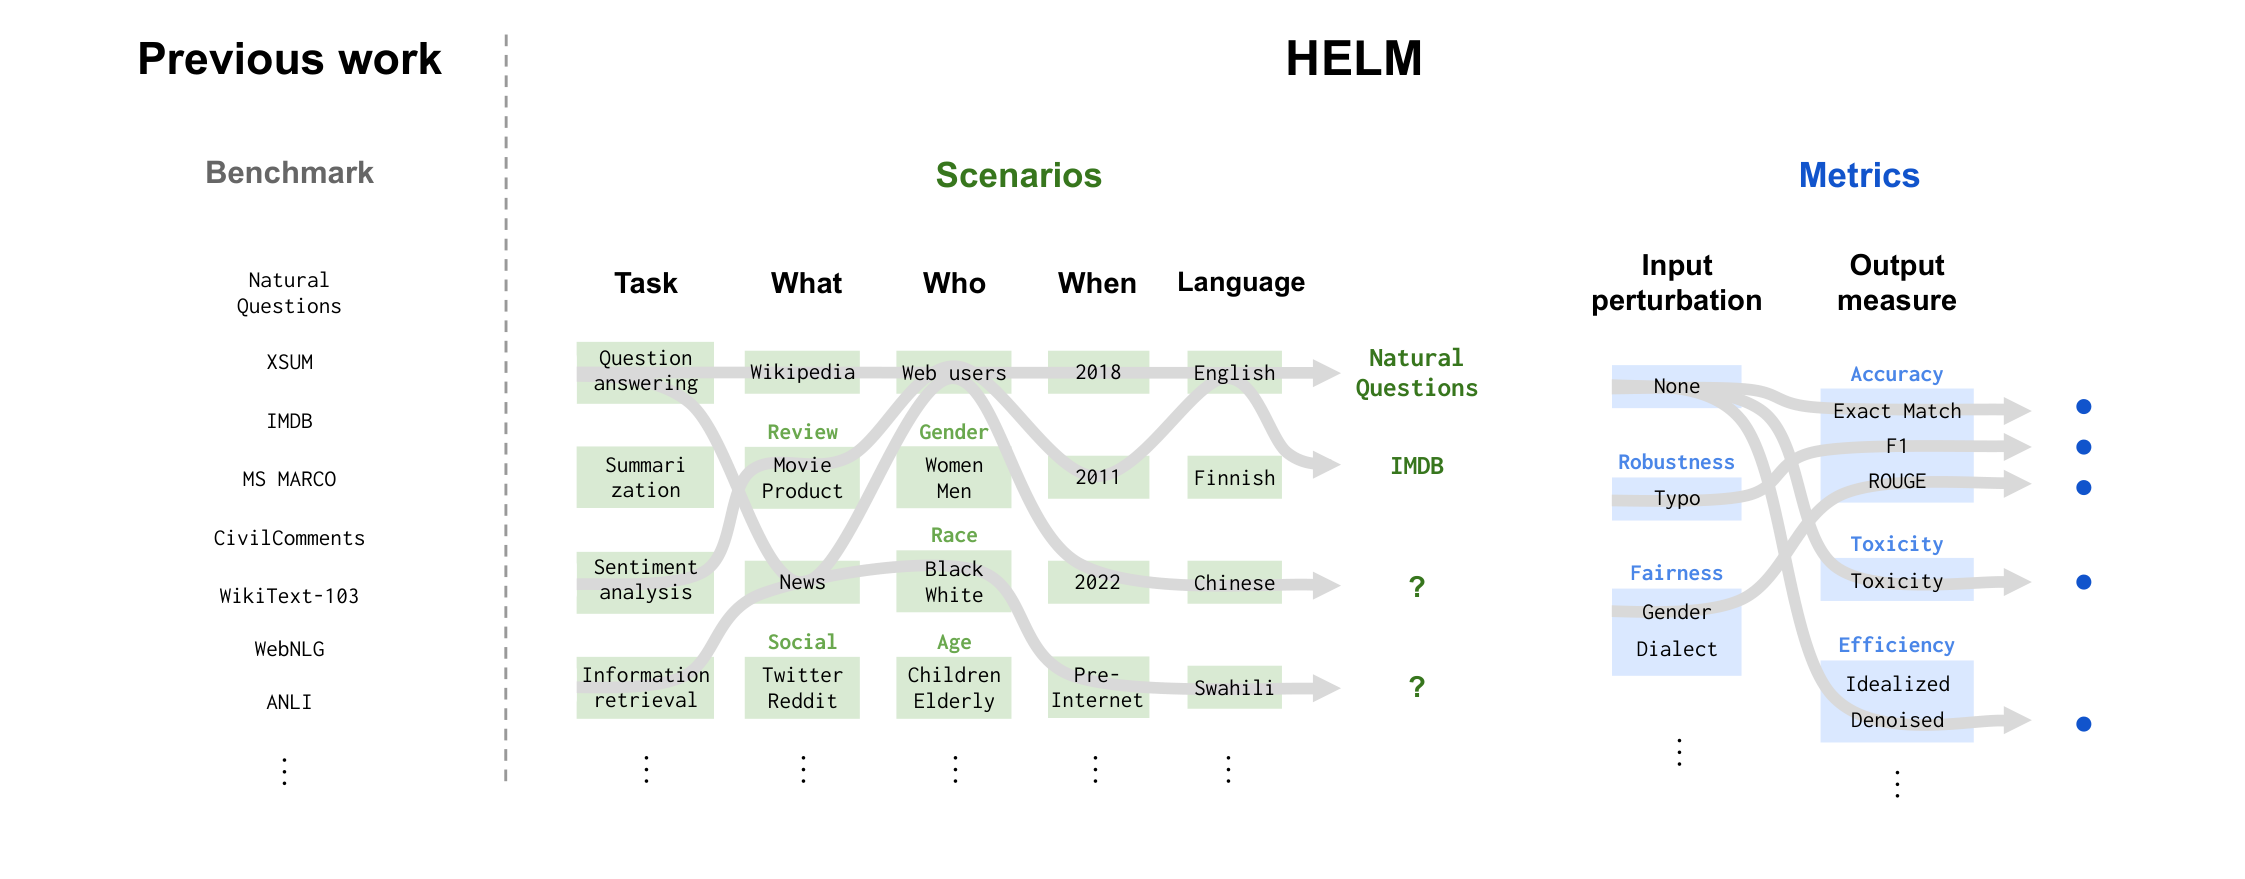
\includegraphics[width=\textwidth,height=0.48\textheight,keepaspectratio]{images/llm-evaluation/helm_fig2_taxonomy_scenarios_metrics.png}\\[0.2em]
  {\scriptsize ``The importance of the taxonomy to HELM.'' Liang et al., ``Holistic Evaluation of Language Models,'' TMLR 2023, \href{https://arxiv.org/abs/2211.09110v2}{arXiv:2211.09110v2}, Figure 2.}
\end{frame}

\begin{frame}{HELM: Standardisation Is the Contribution}
  \begin{itemize}\footnotesize\itemsep0.45em
    \item[\textcolor{red}{$\blacktriangleright$}] HELM evaluates \textbf{30 models} from \textbf{12 organisations} on \textbf{42 scenarios} (16 core $+$ 26 targeted), for \textbf{4{,}939} total runs.
    \item[\textcolor{red}{$\blacktriangleright$}] Seven metrics are measured for each core scenario wherever possible (87.5\% of the time): \textbf{accuracy, calibration, robustness, fairness, bias, toxicity, efficiency}.
    \item[\textcolor{red}{$\blacktriangleright$}] The headline result is about \textbf{coverage}, not ranking: before HELM, models had been evaluated on only \textbf{17.9\%} of the core scenarios; afterwards, \textbf{96.0\%}. Several core scenarios had \textbf{no} model evaluated on them at all.
    \item[\textcolor{red}{$\blacktriangleright$}] The lesson for your own work: most of the value of an evaluation suite comes from running \textit{every} model through \textit{the same} pipeline. Numbers copied from different papers are usually not comparable.
  \end{itemize}
  \vspace{0.15em}
  {\scriptsize Liang et al., ``Holistic Evaluation of Language Models,'' TMLR 2023, \href{https://arxiv.org/abs/2211.09110v2}{arXiv:2211.09110v2}.}
\end{frame}

\begin{frame}{The Eval-Driven Development Loop}
  \begin{columns}[T,onlytextwidth]
    \column{0.44\textwidth}
      \begin{itemize}\footnotesize\itemsep0.4em
        \item[\textcolor{red}{$\blacktriangleright$}] Evaluation is not a phase at the end. It is the loop that everything else runs inside.
        \item[\textcolor{red}{$\blacktriangleright$}] \textbf{Look at traces first.} Almost every useful eval starts as an error you noticed by reading real outputs, not as a metric you chose in advance.
        \item[\textcolor{red}{$\blacktriangleright$}] \textbf{Turn each recurring failure into a test case.} The eval set grows out of production, and it grows in the direction where the system is weak.
        \item[\textcolor{red}{$\blacktriangleright$}] \textbf{Only then automate.} Cheap assertions first, model judges second, humans reserved for the cases that decide the release.
      \end{itemize}
    \column{0.54\textwidth}
      \centering
      \vspace{0.5em}
      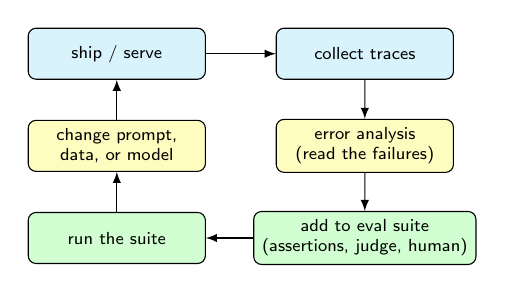
\begin{tikzpicture}[font=\sffamily\scriptsize, >=latex, scale=0.9,
          every node/.style={transform shape},
          box/.style={draw, rounded corners=0.1cm, align=center, minimum width=2.5cm, minimum height=0.72cm},
          d/.style={box, fill=cyan!15},
          m/.style={box, fill=yellow!25},
          e/.style={box, fill=green!18}]
        \node[d] (ship)  at (0,3.0)   {ship / serve};
        \node[d] (trace) at (3.5,3.0) {collect traces};
        \node[m] (err)   at (3.5,1.7) {error analysis\\(read the failures)};
        \node[e] (suite) at (3.5,0.4) {add to eval suite\\(assertions, judge, human)};
        \node[e] (run)   at (0,0.4)   {run the suite};
        \node[m] (fix)   at (0,1.7)   {change prompt,\\data, or model};
        \draw[->] (ship) -- (trace);
        \draw[->] (trace) -- (err);
        \draw[->] (err) -- (suite);
        \draw[->] (suite) -- (run);
        \draw[->] (run) -- (fix);
        \draw[->] (fix) -- (ship);
      \end{tikzpicture}\\[0.4em]
      {\scriptsize Production traces feed the eval suite; the suite then gates every change before it ships.}
  \end{columns}
\end{frame}
